%% This is an example first chapter.  You should put chapter/appendix that you
%% write into a separate file, and add a line \include{yourfilename} to
%% main.tex, where `yourfilename.tex' is the name of the chapter/appendix file.
%% You can process specific files by typing their names in at the
%% \files=
%% prompt when you run the file main.tex through LaTeX.
\chapter{State of the Art}

In this chapter there will be an extensive explanation to the technologies used
throughout the document.

\section{Internet of Things}

What is the \textbf{\textit{Internet of Things}}?\\
\textit{Internet of Things}, better known as IoT, is the world of interconnected devices
connected to the real world and to the Internet. These devices has a very
broad definition, from the smart sensors in a power plant to the smart fridge in
a house. What connects these devices is their ability to be connected with the world,
sharing, with the needed restrictions, their work. This opened the door to a new
revolution in the IT sector, prompting new opportunities for developers, entrepreneurs
and end users. Some of the most relevant endings of these technologies are \textit{Smart Houses},
\textit{Smart Cities}, Cars etc. %[TODO] continue a little bit here

\subsection{Ecosystems}

What is an Ecosystem? An ecosystems is by definition \textit{a system, or a group of interconnected elements,
formed by the interaction of a community of organisms with their environment.},
in our case a set of smart devices connected between them. The IoT world is evolving
from distinct single entities to more evolved clusters of devices which can communicate
more easily between each other.These are usually are made by companies using specific protocols or standards
to simplify the connection between their products, but at the same time closing it to the others.
%[TODO] connect the two paragraphs
The list of products related to the \textit{Internet of Things} is too broad for
being even listed, due to the highly expanding sector related to smart devices.
However we will consider the most common ecosystems which can be easily found in a common
home, meaning services for: Smart Lights, Cameras, Thermostats etc. Luckily
most of them are being bought and integrated in bigger environments run by
famous companies such as \textit{Google} or \textit{Apple}.
The reason for which we try to restrict the integration with these ecosystems is
mainly practical, because they're the most common and they do offer simulators
for testing, and because they suits perfectly our scenario.

\subsubsection{Google - Nest}

\textbf{Nest} is a home automation producer of smart devices
which ranges from their famous Smart Thermostat to the locking system, from the
washing machine to the light system, from the \textit{Dropcamera} to the Hi-Fi Sound system,and
these are just some examples. The number of components supported by this company
is wide, which makes it a good choice to support in our scenario, also because of
the high cost of these devices. The main added value given by these accessories is related
to two main points: saving money with a smart consumption of electricity and the ability
to remotely control the house with an easy to use application.
Besides the commercial value of \textit{Nest}, the platform offers many tools for developers
to interact with their platform using their Cloud service. Third party developers
are encouraged, with some limitations, to use their Cloud service which
offers some \textit{RESTful} APIs to gather access to the remote devices.
The remote access through APIs unlinks developers from platform dependent libraries (see later HomeKit)
that restricts the use or the integration with a specific technology.
Furthermore it is possible to access directly \textit{Nest} devices with their \textit{Nest Wave}
which allows direct communication with non-branded devices using two different communication protocols,
mainly \textbf{802.11} standards.


\subsubsection{Apple - HomeKit}

\textbf{HomeKit} is a very similar ecosystem to the one described before, producing or supporting
home automation devices. \textit{HomeKit} relies on the large network of Apple devices,
making it an environment to be considered even if it is relatively new on the market. The key
point of \textit{HomeKit} is the easy integration with Apple devices, fitting almost perfectly wherever
there was an already existing Apple ecosystem. Developers are allowed to take control of the devices
only through iOS applications, restricting the possibilities of integration with different ecosystems or
technologies. Moreover it ties the developers to their technology making it really hard to be adopted in a different
system. However as we'll see later it is possible to bypass the problem using the microservice architecture to
make the system independent from specific technologies.


\subsubsection{Samsung - SmartThings}

\textbf{SmartThings} is another ecosystem from \textit{Samsungs} with many similarities
with the former producers.\textit{SmartThings} focuses on four main Smart devices categories:
\textit{Security},\textit{Monitoring}, \textit{Lighting and Energy} and \textit{Convenience and Entertainment}.
\textit{SmartThings} as the previous ecosystem does not allow a direct interaction with the smart devices,
but offers a developer-friendly interface to their Cloud Service. However, as \textit{HomeKit} it is tied to
a technology, making it harder for different technology stacks to access.


\section{The Microservice Architectural Style}

\subsubsection{SOA vs Microservices}
In short, the \textit{microservice architectural style} is an approach to developing a single
application as a suite of small services, each running in its own process and communicating with
lightweight mechanisms, often an HTTP resource API. These services are built around business capabilities
and independently deployable by fully automated deployment machinery. There is
a bare minimum of centralized management of these services,
which may be written in different programming languages and use different data storage technologies.[7]\\
There is a close link between the \textit{microservice architecture} and the \textit{service oriented architecture},
thus due to their nature the community classified microservices as a subclass of the service oriented architecture.
\textit{Don Box} of Microsoft described the Service-Oriented paradigm with the following four principles [8]

\begin{enumerate}
  \item Boundaries are explicit
  \item Services are autonomous
  \item Services share schema and contracts, not class
  \item Service compatibility is based on policy
\end{enumerate}

Microservices fullfills the first two requirements, with a very strong focus on the second principle.
However the functionalities are very frequently exposed using a \textit{RESTful} interface, which
doesn't expose any contract nor schema. Furthermore microservices holds another subtle difference related to their
scope, where a microservice serves as a service inside its application meanwhile typical SOA services
serves a broader scope and \textit{can be} part of the same application.
The difference between the two concepts is very subtle, and it wouldn't be impossible for them
to be the same in certain situations. \textit{Bob Ruhbart} from Oracle described shortly the difference:
\textit{Microservices are the kind of SOA we have been talking about for the last decade. Microservices must be independently deployable,
whereas SOA services are often implemented in deployment monoliths.
Classic SOA is more platform driven, so microservices offer more choices
in all dimensions}.[10]

\begin{figure}[h]
\caption{Graphic illustration of microservices and SOA}
\centering
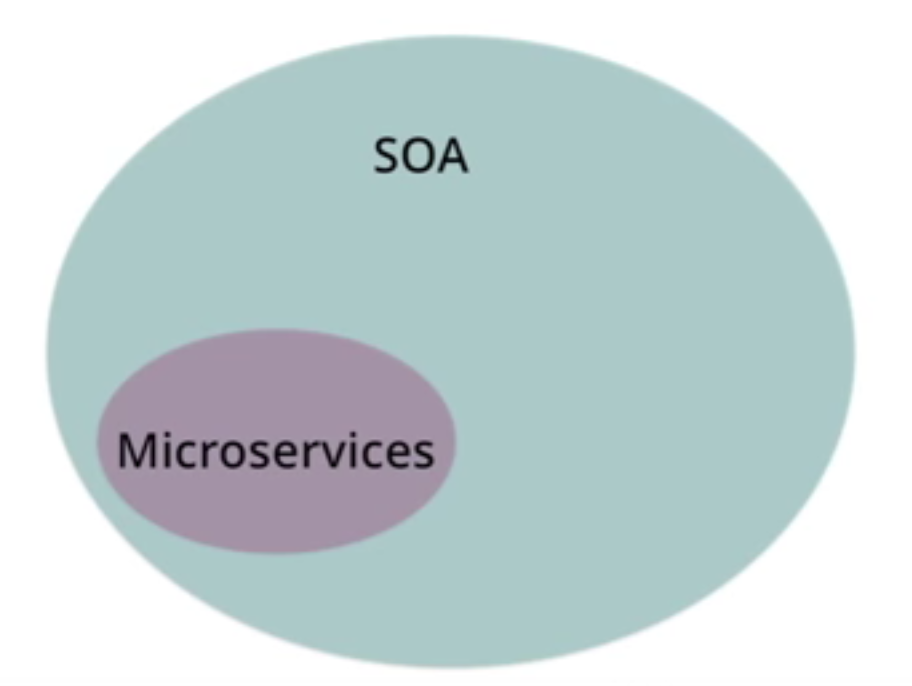
\includegraphics[scale=1]{soavsmicro.png}
\end{figure}

\subsection{Internal integration}
Typically when a new component has to be added to an existing
project the approach consists in the development of a library which
has the logic to deal with the new module to be supported. Subsequently the component
will
become part of the project itself, with its needs to be updated throughout time.
However when the number of components to integrate increases it will affect the size
of the project and very likely its performances.
In our case the component to be integrated will be the ecosystem driver,
having a set of libraries which are capable of interacting with the remote APIs or
with the direct wired connections. As we'll see in the next paragraph this is a typical
monolith approach, meanwhile for this situation would be better to use a microservice approach.

\subsection{Integration as a Service}
Considering the \textit{Microservice} architectural pattern we can decompose
the above situation creating dedicated services capable of handling the
required business logic to interact with an external system. This approach
is also called \textbf{Componentization via Services}[7], where a component is defined
as a \textit{unit of software that is independently replaceable and upgradeable.}
It is important to distinguish between \textit{libraries} and \textit{services}:
the latter uses out-of-service components to communicate, mainly HTTP requests or
remote procedure calls when libraries uses instead mechanisms like in-memory calls.
The main advantage to build components as services instead of libraries is the
possibility to deploy them individually without the need to redeploy the whole system.
If a library is modified or removed the whole system will need to be redeployed,
which in most of the cases it is converted in a loss of money and time. That's not
the case if the system is composed by many independent systems, where only the changed
service will need a new deployment. However this is not always true, there will be some
circumstances where it will be necessary anyway to deploy again the whole system, but the
aim of this approach is to reduce the number of these necessities.

\subsection{Other benefits}
Apart from the benefits already listed formerly, there are other benefits introduced by
adopting the microservice architecture:

\begin{description}
  \item[Heterogeneity between technologies] Structuring the system as a set
  of services frees us from the limitations of a singular technology allowing
  us to adopt different frameworks for different tasks. This benefits on the
  possible optimization that can be achieved using the right technology for the
  right task. Furthermore this removes completely the problem of creating adapters
  for different technologies to integrate in the system if they do not exist. This is
  also called \textbf{Decentralized Governance}.
  \item[Evolutionary Design] is a concept popularized by the \textit{Extreme Programming},
  where the system is continuously evolving during the phases of it's development.
  This key feature makes possible to evolve adopting a microservice architecture while
  keeping the old legacy monolith system, well tested and functional, without rewriting
  the whole system.
  \item[Designed for failure] Building a system made of services instead of components
  leads the developers to take more effort in considering failures. Developers have
  to take in consideration the possible failure while reaching the service, and
  prevent the system to crash and handle the situation in the most gentle way. On the
  other side, this approach introduces more overhead to handle the possible situations.


\end{description}


\subsection{Microservice Oriented Internet of Things}
IoT with their advent brought up some, not yet resolved, challenges which fits
very well with the Microservice architecture. \textit{Interoperability} is one of these
challenges aimed to be solved. Microservices \textit{decentralized governance} feature,
which allows the use of different technologies inside the same systems holds the key for
solving the interoperability problem. Key IoT devices vendors realizes that if their products
supports multiple interoperability standard they're likely to be adopted also by their
competitors (e.g. Nest products are available on HomeKit).[3] Microservices here can be
used as isolated adapters for the many different technologies, facing the spreading
fragmentation of communication protocols between machines.\\
Microservices are by nature dynamic and reactive, which makes them a good choice for
an environment where new technologies are frequently added or modified.

\section{Calvin}
  \textit{Calvin} is an Open-Source distributed framework designed mainly, but not only,
  for IoT systems. The key point of \textit{Calvin} is the "Distributed cloud for IoT", meaning
  running the code where it best suits the performance needs, a crucial aspect since we are
  dealing with low-resource components. We will use \textit{Calvin} for the whole course of the document,
  referring to it as the main "system", also used to integrate with the others. \\
  \textit{Calvin} has the ability to integrate new components without replacing them by writing
  proxies for the specific hardware to support. Proxies are actors written to handle
  communication with the legacy system. Such a proxy actor handles the task of converting data
  from the application into messages or requests the old system can handle, and converting the
  response back into tokens the Calvin application understands.[14]

        \begin{figure}[h]
        \caption{Proxies interaction}
        \label{fig:calvinproxy}
        \centering
        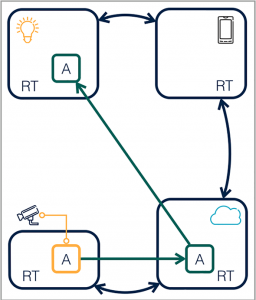
\includegraphics[scale=0.75]{calvin4.png}
        \end{figure}
  Figure \ref{fig:calvinproxy} shows the interaction of native Actors and Actors which
  acts as a proxy for legacy components, in this example the camera.




  \textit{Calvin} is built upon the well-established actor model, using a methodology often referred to as dataflow programming[11], and
  its life cycle can be summarized in four, well-distinct, phases: \textit{Describe}, \textit{Connect}, \textit{Manage}
  and \textit{Deploy}.

\subsection{Describe}
  The smallest functional units in \textit{Calvin} is an Actor. Actors do not share
  nor state or behavior, encapsulating all the logic. The key point of Actors in Calvin
  is their reactivity: they react to external events or when receiving inputs. Actors
  communicates only using data through ports, has to be defined before deploying the system.
  This way is possible to describe the possible interactions that the actor may have when
  connecting it to others.\\
  Having a non-shared internal state allow the Actor to be serialized and moved to another
  running machine or to be backed up if the machine crashes. However this is partly true because
  it may be tricky to serialize Actors with a very complex internal state.

  \begin{figure}[h]
  \caption{Describe Phase}
  \centering
  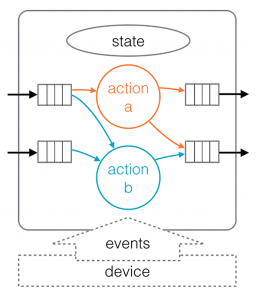
\includegraphics[scale=0.75]{calvin1.png}
  \end{figure}


\subsection{Connect}

    \begin{figure}[h]
    \caption{CalvinScript Example}
    \label{fig:calvinscript}
    \centering
    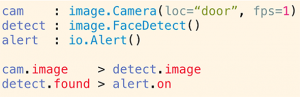
\includegraphics[scale=0.75]{calvin2.png}
    \end{figure}

  After describing the many functionalities provided by the various Actors in the system
  we need to tie them to build applications. \textit{Calvin} offer a scripting language,
  named \textbf{CalvinScript}, to describe the various connections between actors
  and their input and output ports. In figure \ref{fig:calvinscript} there is an example
  of a script for detecting faces in an image. The first part is relative to the actors declaration
  and initialization, giving a clear description of which actors will be playing in the current
  environment. The second part describes the links between each actors, structuring the flow
  of the process. In this case the actors in the system are 3: the \textit{Camera}, the \textit{Detector}
  and the \textit{Alert}. The flow of the process is relatively simple in this case, and it is structured
  as follows: the  \textit{Camera} takes a picture, which will be passed to the \textit{Detector}. Subsequently
  the \textit{Detector} will send its result to the \textit{Alert} actor, which will possibly fire an "alarm" if he
  detects any human face inside the picture.\\
  Figure \ref{fig:calvinactors} shows a more complex interaction between actors. %%[TODO] maybe add something here about the picture

  \begin{figure}[h]
  \caption{Actors interaction}
  \label{fig:calvinactors}
  \centering
  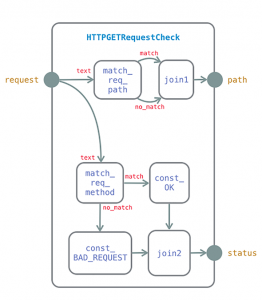
\includegraphics[scale=0.75]{calvin3.png}
  \end{figure}



\subsection{Deploy}

  Each Actor has different resource requirements needs to be satisfied in order to be
  deployed successfully. For example, referring to the previous scenario, an actor
  using a camera needs to be deployed on a system where there actually is a camera. These
  are also called \textit{hard} or \textit{unconditional requirements}, which determines
  the possibility to instantiate or migrate the actor on a machine. \\
  On the other side there are also \textit{non-functional requirements}, describing where
  an actor would suit best for its task. Always referring to the former example, when applying
  face detection it would be better to perform this task on a more performing machine compared to
  a low-resource machine, like a \textit{Raspberry Pi}.\\
  However at the moment \textit{Calvin} supports only \textit{static deployment}, needing the user
  to define where to deploy and execute the actors.

\subsection{Manage}
  When the whole runtime is running it is more than needed to have a tool to keep
  track and monitor the activities in the system. The runtime can be queried to retrieve
  informations about the actors and locate them. It is also possible to track
  the actors firings, on which ports and step by step execution. These are mainly
  debugging tools, though it is also true that this is a recent framework and many
  functionalities are already in development.

 %%[TODO] add description of the Calvin layers (actor, calvinsys, runtime)

\subsection{The relationship between the Actor Model and Microservices}
Actors are isolated, single-threaded components that encapsulates both state and behavior.
Typically actors communicates using lightweight direct messaging systems, for example
to receive or return inputs/parameters. Microservices are very similar to Actors in many
of their key aspects, such as isolation, encapsulation and lightweight messaging, though
usually microservices uses RESTful interfaces. There is some discussion
in the community whether some argues that actors are actually microservices
themselves [12] meanwhile others defines actors as a subset of microservices[13].
This however heavily depends on the actors framework adopted for the situation, which in our
case an Actor can not be compared to a microservice due to an insight limitation: \textbf{Calvin Actors can not
use different technologies}, at the moment.
